% !TEX root = main.tex

All participants completed the task (40 trials in total). Average trial duration was 186s (SD 18.2s, min 162.2s, max 300.1s). Average number of collisions was 17.8 (SD 4.9, min 5, max 40). Average trial velocity ranged between 1.37 and 2.54 units per step (mean 2.23, sd 0.19). Maximum instantaneous speed was 3.6 and minimum 1.06. The supplementary information provides comprehensive data on performance-related features, such as trial duration, along with correlations between them; also it includes further details on participant self-report and background, plus validation of our main result for {\sf RQ2}.


\subsection{RQ1: How does performance change over time?}

What is the form of the learning curve, does it consistently improve e.g. as a power law of practice \citep{Newell1982}? A power-law curve transformed to log-space will be linear. Thus, to investigate whether participant behaviour follows a power law, we fitted a linear model in log-log space (log-transformed dependent and independent variable) of trial durations as a function of cumulative number of trials, for each participant separately. Fig.~\ref{fig:flowVperf} (panel A) shows this log-log performance data for each participant in each trial. Blue dashed lines indicate the power-law LC. Distance of points from the line (residuals) indicate the deviation of each trial from predicted learning: points above the line indicate longer duration (worse performance) than predicted by the LC, and vice versa.

\begin{figure}[!p]
	\centering
	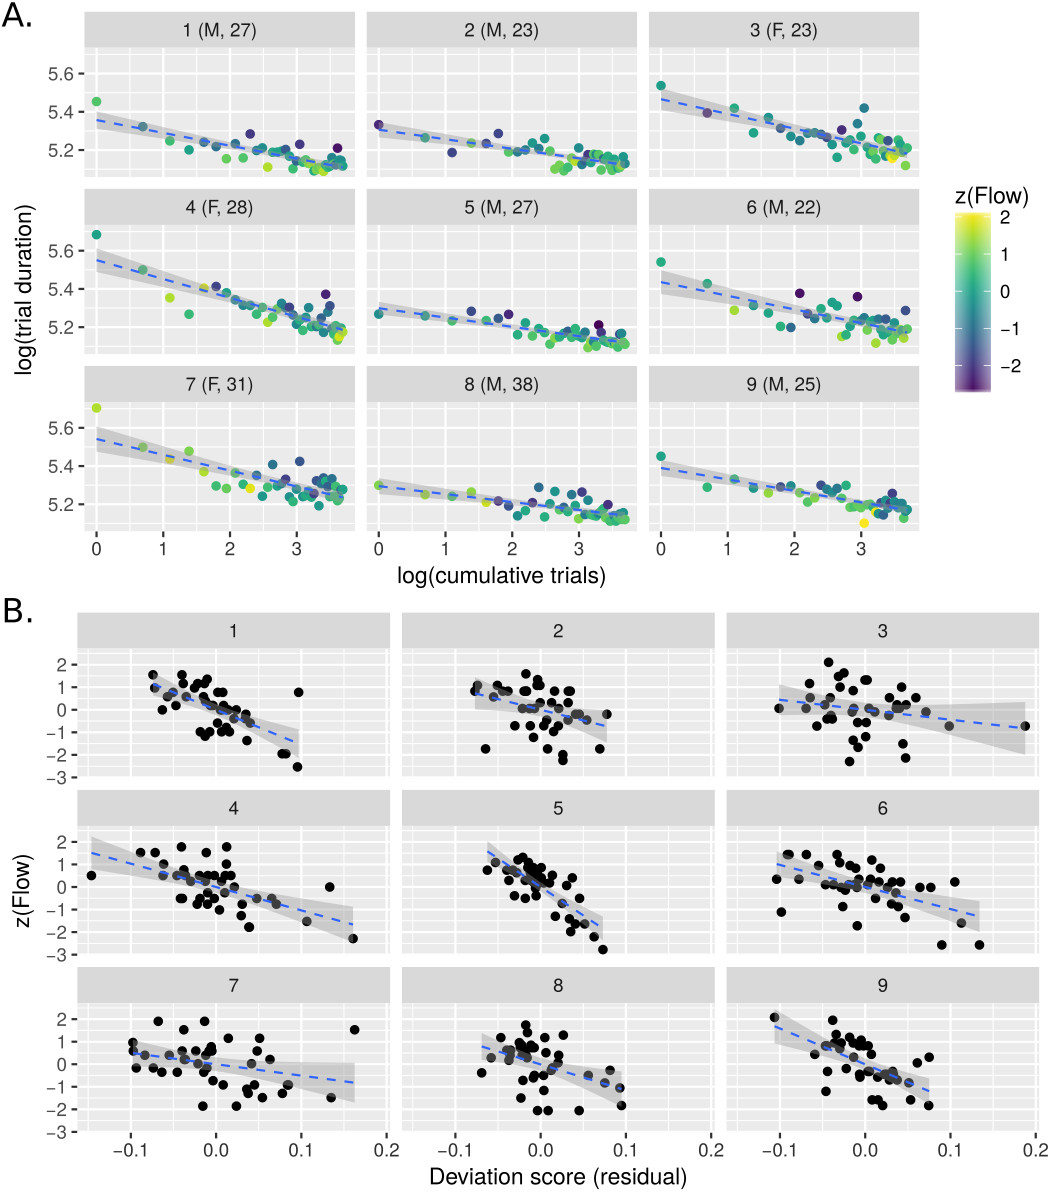
\includegraphics[width=\linewidth]{cogcar_main}
	\textbf{\refstepcounter{figure}\label{fig:flowVperf} Figure \arabic{figure}.}{{\it Panel A}: Participant-wise data showing logarithm-transformed performance and Flow self-reports in the speeded steering task. Ordinate shows log-duration of trials, abscissa shows log-cumulative trial count. Dashed blue lines fitted to the data are power-law learning curves, which transform to linear in log-log space. 95 \% confidence intervals around the slope are greyed.\\
	{\it Panel B}: Participant-wise deviation scores (observed trial duration minus predicted trial duration) plotted against Flow scores for each participant, and fitted by linear models. 95 \% confidence intervals around the slope are greyed.}
\end{figure}

All participant-specific log-log models had negative slopes, which indicates that with experience each participant learned to play better (obtained faster trial times). The variation in intercepts reflects disparity in participants' initial skill levels, and the variation in slopes the different learning rates. The individual intercepts and slopes of the models are presented in Table~\ref{tab:LCxFlow}. A grand model was also fitted for all participants, and cumulative number of trials explained 39.6\% of variance in trial durations. As the performance generally improves with cumulative trials, in agreement with a power-law of learning model, the explained variance can be ascribed to learning.

To confirm that a power law model gives a good approximation of learning, we compared its model-fit criterion against the fit of an exponential curve model (see Supplementary Information for details). While both models had good fit, the power law model was slightly better.

RQ1 can thus be answered: {\it the task was learned and the LC fit well to a power law model}. Given these positive answers, we may assume that the model provides a useful statistical estimate of performance expectation, i.e. how well the participants expect to perform can be estimated from the model.

\begin{table}[ht]
	\centering
	\textbf{\refstepcounter{table}\label{tab:LCxFlow} Table \arabic{table}.}{Individual learning rate parameters (cols 2--4), Flow (cols 5--6) and perceived importance (P.I., cols 7--8) scores. Last row shows group-mean values of each column.}
	\begin{tabular}{llllllll}
	\hline
	Participant & Intercept sec & Intercept log & Slope  & Flow mean & Flow SD & P.I. mean & P.I. SD \\
	\hline
	1           & 213     & 5.36      & -.067 & 5.10      & .51     & 3.53      & .57     \\
	2           & 202     & 5.31      & -.049 & 5.18      & .39     & 4.29      & .47     \\
	3           & 237     & 5.47      & -.077 & 5.36      & .64     & 2.03      & .50     \\
	4           & 257     & 5.55      & -.099 & 4.40      & .39     & 4.12      & .46     \\
	5           & 200     & 5.30      & -.049 & 5.44      & .88     & 5.16      & .64     \\
	6           & 230     & 5.44      & -.071 & 5.22      & .82     & 4.33      & .56     \\
	7           & 255     & 5.54      & -.083 & 4.69      & .53     & 2.22      & .53     \\
	8           & 198     & 5.29      & -.041 & 4.94      & .90     & 3.67      & .70     \\
	9           & 219     & 5.39      & -.059 & 5.25      & .79     & 4.62      & .55     \\
	\hline
	Group mean  & 223     & 5.41      & -.066 & 5.06      & .65    & 3.77      & .55    \\
	\hline
	\end{tabular}
\end{table}

%           tests  pvals   padj
% 1       LCxFlow 0.0800 0.6400
% 2      FlowXssn 0.7700 1.0000
% 3  FlowXssn1dur 0.9000 1.0000
% 4  FlowXssn2dur 0.9000 1.0000
% 5  FlowXssn3dur 0.0300 0.3000
% 6  FlowXssn4dur 0.0200 0.2200
% 7  FlowXssn5dur 0.9000 1.0000
% 8  FlowXssn6dur 0.0300 0.3000
% 9  FlowXssn7dur 0.9000 1.0000
% 10 FlowXssn8dur 0.9000 1.0000
% 11 FlowXssn9dur 0.9000 1.0000
% 12     FlowXdev 0.0002 0.0024
\subsection{RQ2: How is Flow related to performance?}

% data:  Flow and LC (from table 1)
% t = 2.0678, df = 7, p-value = 0.07747
% alternative hypothesis: true correlation is not equal to 0
% 95 percent confidence interval:
%  -0.08177327  0.90840927
% sample estimates:
%       cor
% 0.6157904
Participant-wise mean Flow and LC slope were related but not significantly correlated (Pearson's correlation coefficient {\it r} = 0.6, {\it p} = 0.6, N = 9). %NHST1
Since we have established that performance improves over sessions, we also used session number as a simple proxy of performance improvement. Fig.~\ref{fig:FlowVssn} shows the group-wise distribution of Flow scores plotted against sessions: clearly, there is no effect of session on group-wise median Flow (Pearson's {\it r} = -0.12, {\it p} = 1.0, N = 8).%NHST2

\begin{figure}[!b]
\begin{center}
	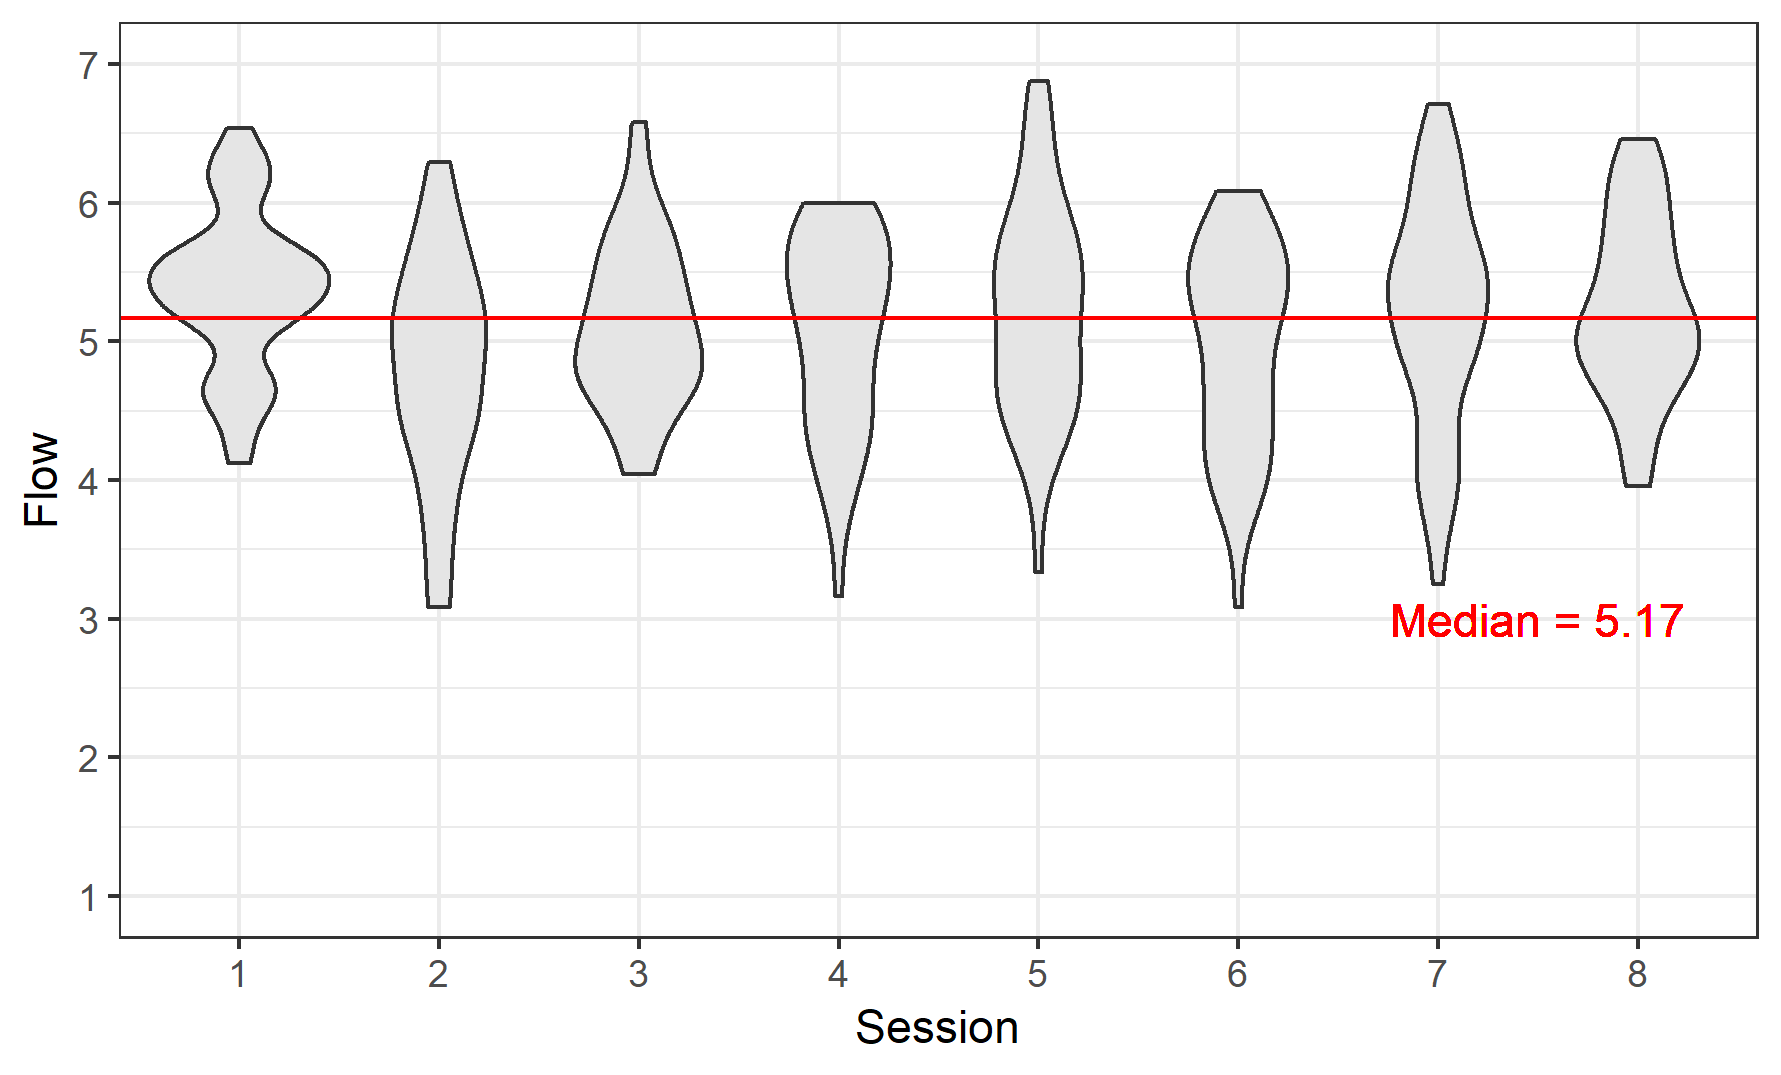
\includegraphics[width=\nicewidth]{session_fss2}
\end{center}
	\textbf{\refstepcounter{figure}\label{fig:FlowVssn} Figure \arabic{figure}.}{Violin plot representing participants' self-reported Flow in sessions 1-8 (per-session Flow = mean of five trials. The self-report items are given in Supplementary information, the scale was 1-7).}
\end{figure}

Next, we calculated the group-wise correlation of median duration and median Flow, separately for each session. The relationship between duration and Flow was intermittently significant {\it before correction for multiple comparisons}, but not after, and with no particular trend (range of Pearson's {\it r} = [-.05 $\dots$ -.74], {\it p} = [0.2 $\dots$ 1.0], N=9 for all). These results suggest that higher Flow was sometimes associated with lower trial durations (i.e. better performance), but not strongly and not systematically. If we group sessions by condition (introduction=1, practice=2--4, main test=5--8), we can visualize the evolution of performance against Flow more clearly than by plotting each session individually, see Fig.~\ref{fig:FlowVdurXssn}.%NHST3-11

\begin{figure}[!t]
\begin{center}
  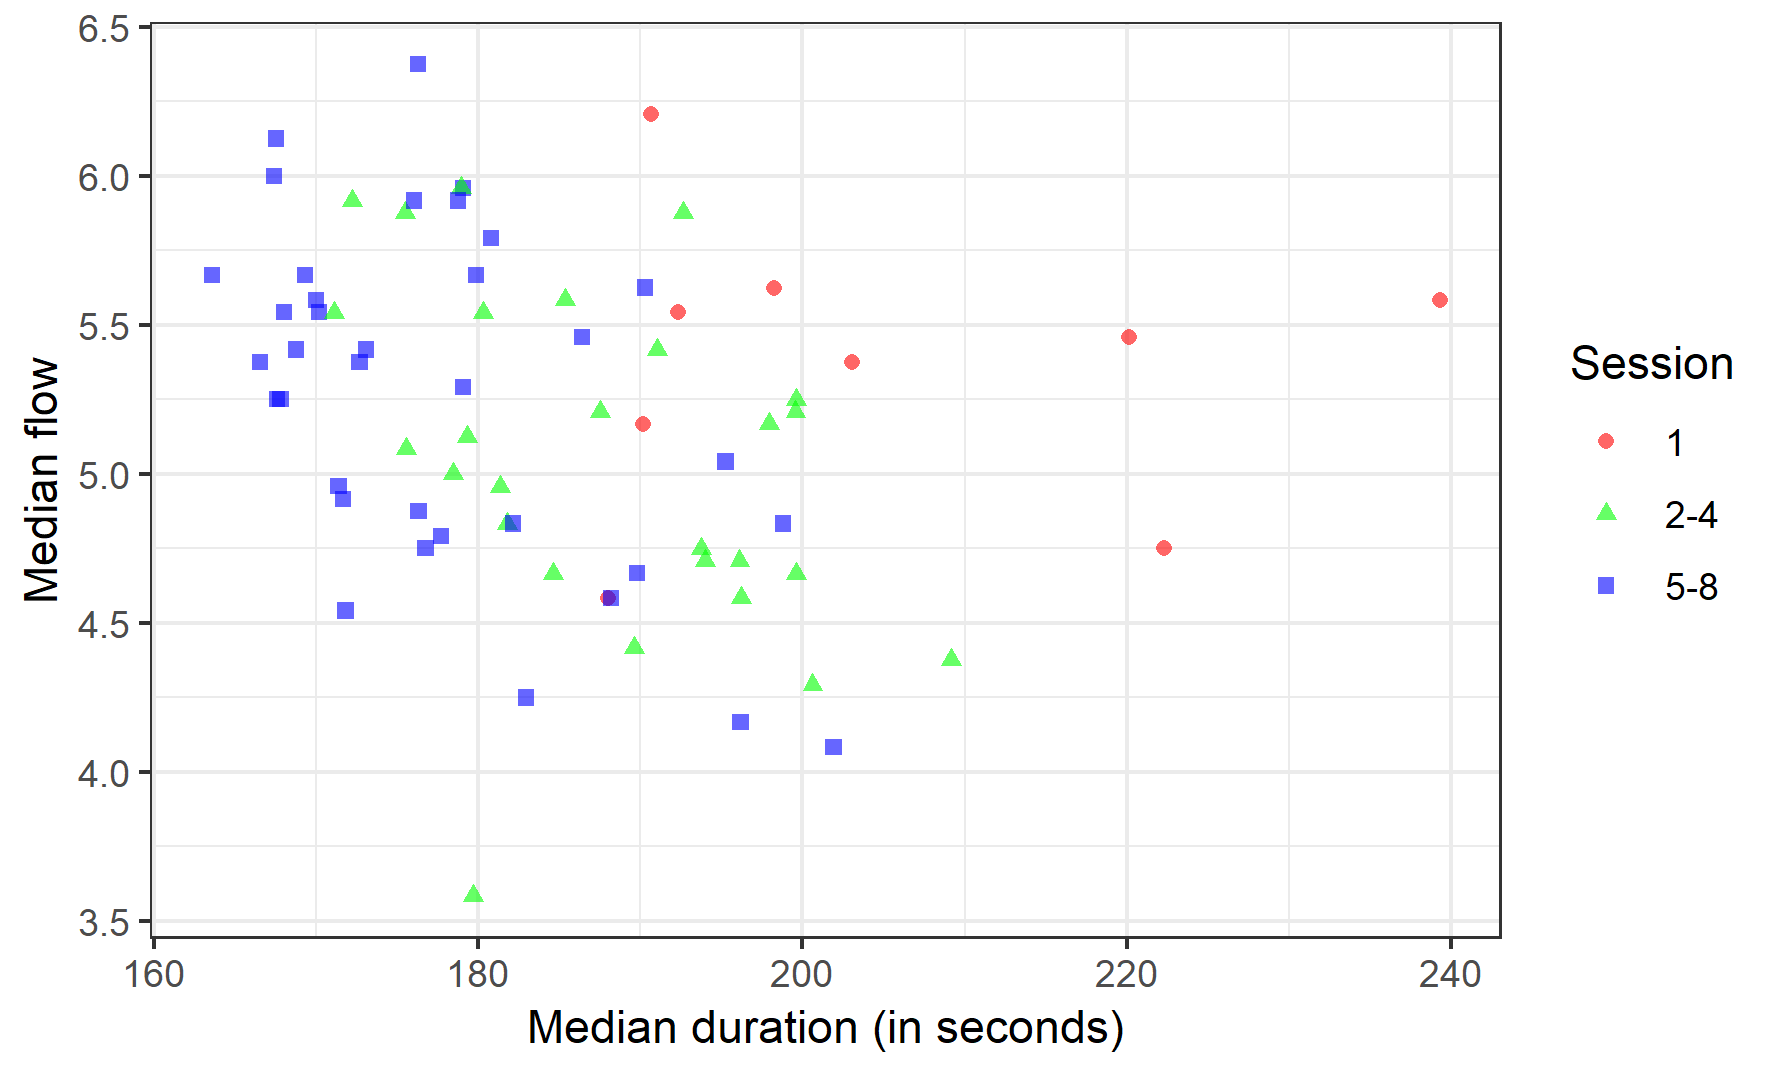
\includegraphics[width=\nicewidth]{session_flowDuration_v3}
\end{center}
  \textbf{\refstepcounter{figure}\label{fig:FlowVdurXssn} Figure \arabic{figure}.}{Duration and Flow over sessions grouped: 1 (Introduction+physiological measurements), 2-4 (training), 5-8 (physiological measurements), N = 72.}
\end{figure}

The relationships between global (over all responses) Flow and performance appear weak, but we also wish to examine local Flow for each trial separately. The points in each subplot of Fig.~\ref{fig:flowVperf} (panel A) are coloured according to Flow self-reports made after each trial, in a standardised range (original scores transformed to {\it z}-scores). The highest Flow scores are green, the lowest are red. Interestingly, this figure reveals at a glance that the points lie above and below the log-transformed power-law line in good agreement with the level of experienced Flow: worse performing trials (data-point above the line) tend to be more red (Flow scores below the participant-wise mean), and better performing trials tend to be more green (scores above the mean). In other words, it seems that whenever participants were performing {\it better than predicted by the power-law line}, they were experiencing more Flow, and {\it vice versa}.

We evaluated whether this effect was robust and statistically significant. For each participant, we correlated their {\it deviation scores} (signed residuals from the power-law model) with their Flow scores, using a linear mixed model (see Methods). This model was statistically significant (deviation score $\beta$ = -8, {\it t} = -4.36, {\it p} = .002) %NHST12
and the relationship is shown in Fig.~\ref{fig:flowVperf} (panel B; Flow scores are standardized). The conditional pseudo-$R^2$ value for this model was .47, corresponding to a correlation of ~.68, so that the model explains $\sim$47\% of Flow score variability.

Thus, {\it high Flow scores are associated with better than predicted results} (trial durations below the predicted performance line), and {\it vice versa}. The strength of this association per participant follows from the strength of the correlation, and overall the model has large effect size.

As can be seen in Fig.~\ref{fig:flowVperf} (panel B), the trend was clearly negative for 7 out of 9 participants, while for two participants, 3 and 7, the trend was similar but the relationship was weaker. Notably, these two participants also reported lower scores on perceived importance: mean scores for these participants were 2.03 and 2.22, whereas the overall mean was 3.77 (see Table ~\ref{tab:LCxFlow}). However, the group-wise interaction between perceived importance scores and deviation scores was not statistically significant.

RQ2 can thus be answered: Flow was not consistently and robustly related to improvement in task performance with the skill acquisition occurring over 2 h of practice. It was, however, consistently related to whether performance was {\it better (or worse) than predicted} given the participant LC. Moreover, this effect might be moderated by self-reported perceived importance of the steering task (more data would be required to clarify).
